\documentclass[a4paper]{article}
\usepackage[utf8]{inputenc}
\usepackage[spanish, es-tabla, es-noshorthands]{babel}
\usepackage[table,xcdraw]{xcolor}
\usepackage[a4paper, footnotesep = 1cm, width=20cm, top=2.5cm, height=25cm, textwidth=18cm, textheight=25cm]{geometry}
%\geometry{showframe}

\usepackage{tikz}
\usepackage{amsmath}
\usepackage{amsfonts}
\usepackage{amssymb}
\usepackage{float}
\usepackage{graphicx}
\usepackage{caption}
\usepackage{subcaption}
\usepackage{multicol}
\usepackage{multirow}
\setlength{\doublerulesep}{\arrayrulewidth}
\usepackage{booktabs}

\usepackage{hyperref}
\hypersetup{
    colorlinks=true,
    linkcolor=blue,
    filecolor=magenta,      
    urlcolor=blue,
    citecolor=blue,    
}

\newcommand{\quotes}[1]{``#1''}
\usepackage{array}
\newcolumntype{C}[1]{>{\centering\let\newline\\\arraybackslash\hspace{0pt}}m{#1}}
\usepackage[american]{circuitikz}
\usetikzlibrary{calc}
\usepackage{fancyhdr}
\usepackage{units} 

\graphicspath{{../Ejercicio-1/}{../Ejercicio-2/}{../Ejercicio-3/}{../Ejercicio-4/}}

\pagestyle{fancy}
\fancyhf{}
\lhead{22.01 Teoría de Circuitos}
\rhead{Mechoulam, Lambertucci, Rodriguez Turco, Londero, Galdeman}
\rfoot{\centering \thepage}

\begin{document}

\section{Comportamiento de Amiplificadores Operacionales.}

\subsection{Introducción}
En el presente punto se analizarán las limitaciones del amplificador operacional  \textbf{LM324} en las configuraciones inversora y no inversora.
\begin{center}  \textbf{Habria que hablar un toque mas aca.} \end{center}
 Hablar de: Que es un polo dominante, relzacion entradaa salida avol fininito e infinito.
GBP=Wp*G
\subsection{Configuración inversora.}
El circuito propuesto por la catedra el cual será trabajado es el siguiente:

\begin{figure}[htb]	
	\centering
	\includegraphics[width=0.7\textwidth]{Ejercicio1/Imagenes/Circuitoinversor.PNG}
	\caption{Configuración inversora.}
	\label{fig:ConfInv}
\end{figure}
Para este punto se obtuvieron los siguientes datos de la hoja de datos del opamp:
\begin{table}[H]
\begin{center}
\begin{tabular}{|c|c|c|c|c|}
\hline
\multicolumn{5}{|c|}{\textbf{Datos}}                                      \\ \hline
\textbf{$A_{vol}$} & Max$V_{in}$ & $V_{cm}$ & Slew rate             & GBW \\ \hline
100 k              & 32V         & VCC-1.5  & 0.3 $\frac{V}{\mu s}$ & 1M  \\ \hline
\end{tabular}
\end{center}
\end{table}

\subsubsection{Calculo Analítico del Circuito.}
Lo primero que se hizo fue utilizar el equivalente de thevenin.\\

\begin{figure}[htb]	
	\centering
	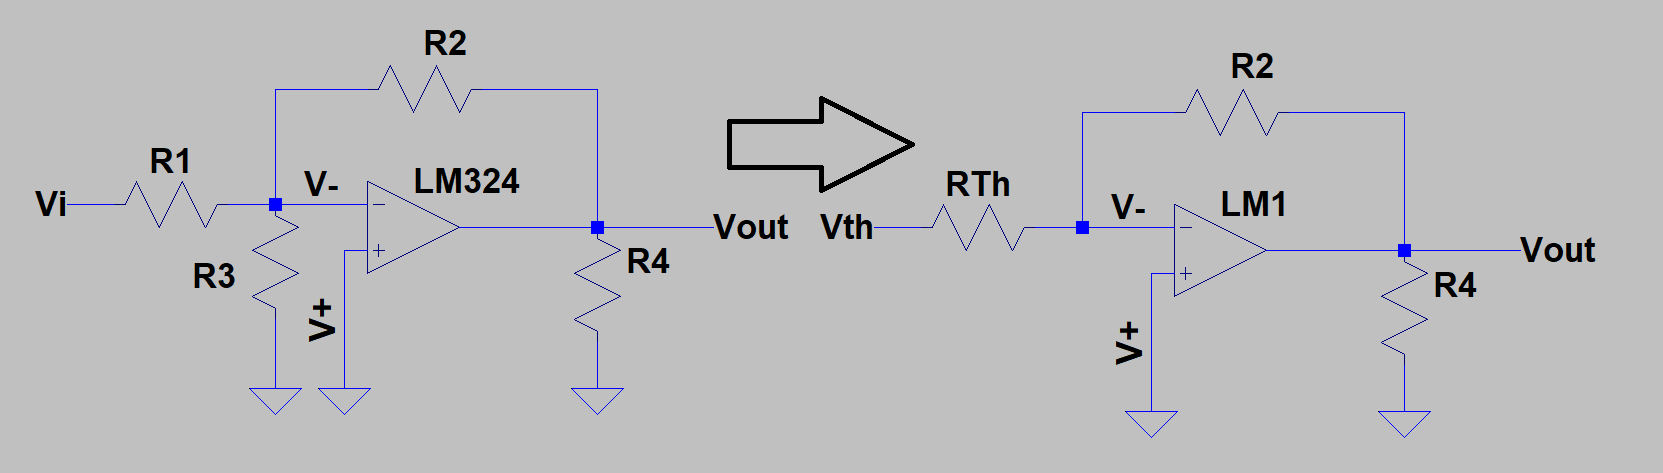
\includegraphics[width=0.7\textwidth]{Ejercicio1/Imagenes/Thevenin.PNG}
	\caption{Aplicacion teorema de Thevenin.}
	\label{fig:Thevenin}
\end{figure}

Luego de esta transformación es mas sencillo realizar los calculos analíticos.
Teniendo en cuenta que 
\begin{align}V_{Thevenin} = V_{in} \cdot \frac{R_3}{R_1+R_3}  \thinspace  R_{Thevenin} = \frac{R_1\cdot R_3}{R_1+R_3}
\label{eq:thev}
\end{align} 

El cálculo se realizara para el caso generico y una ves terminado el desarrollo se tomaran las aproximaciones para los diversos escenarios pedidos.
\begin{align}
V_{Out}= A_{Vol}(\omega) \cdot (V^+ - V^-)
\end{align}
\begin{align}
V^+=0\end{align}
\begin{align}\frac{V_{Th}-V^-}{R_{Th}}=\frac{V^--V_{Out}}{R_2}
\label{eq:nodeInv}
\end{align}
Despejando para $V_{Out}$ se llega a que:
\begin{align}
\label{eq:Vout}
V_{Out}=-V_{in} \cdot \frac{R_3}{R_1+R_3} \cdot \frac{\frac{R_2}{R_{Th}+R_2}\cdot A(\omega)}{1+\frac{R_{Th}}{R_{Th}+R_2}\cdot A(\omega)}
\end{align}
Teniendo en cuenta que la transferencia será $ H(s)=\frac{V_{Out}}{V_{in}}$.\\
Para el caso de $A_{Vol}=\infty$ simplemente bastará con tomar:
\begin{align}\lim_{A_{Vol}\to\infty} - \cdot \frac{R_3}{R_1+R_3} \cdot \frac{\frac{R_2}{R_{Th}+R_2}\cdot A(\omega)}{1+\frac{R_{Th}}{R_{Th}+R_2}\cdot A(\omega)} = -\frac{R_3}{R_1+R_3}\cdot\frac{R_2}{R_{Th}}=-\frac{R_2}{R_1}\end{align}

Para el caso de $A_{Vol}$ finito solamente se reescribira la ecuación \ref{eq:Vout}.

\begin{align}
H(s)= -\frac{R_2\cdot A_{Vol}}{R_1\cdot R_3+R_1\cdot R_3 \cdot A_{Vol} +R_2\cdot R_3+R_2\cdot R_1}
\label{eq:AvolFinite}
\end{align}

Finalmente el caso el cual incluye el polo dominante bastará con tomar 

\begin{align}A_{Vol}(\omega)=A_0 \cdot \frac{1}{1+\frac{s}{\omega'}}
\label{eq:PoloDom}
\end{align}
Donde $\omega'$ es la frecuencia del polo dominante.\\
Utilizando las ecuaciones (\ref{eq:AvolFinite}) y (\ref{eq:PoloDom})
Se llega a la expresión:
\begin{align}
\label{eq:polodom}
H(s)=-\frac{A_0R_2R_3}{A_0R_1R_3+R_1R_2+R_1R_3+R_2R_3} \cdot\frac{1}{1+\frac{s}{\omega' \cdot \frac{A_0R_1R_3+R_1R_2+R_1R_3+R_2R_3}{R_1R_2+R_1R_3+R_2R_3}}}
\end{align}

De la ecuación \ref{eq:polodom} se obtiene la frecuencia de corte del sistema.
\begin{align}
f_c=\frac{\omega'}{2\pi} \cdot \frac{A_0R_1R_3+R_1R_2+R_1R_3+R_2R_3}{R_1R_2+R_1R_3+R_2R_3}
\end{align}
Teniendo en cuenta que
\begin{align}
\omega'=\frac{GBW}{A_0} = 10Hz
\end{align}

Para nuestro grupo los valores de resistencias fueron los del siguiente cuadro:
\begin{table}[H]
\begin{center}
\begin{tabular}{|c|c|c|c|}
\hline
\textbf{Caso:}              & \textbf{1}               & \textbf{2}               & \textbf{3}                \\ \hline
$R_1=R_3$                   & 7k5                      & 7k5                      & 75k                       \\ \hline
$R_2$                       & 75k                      & 7k5                      & 7k5                       \\ \hline
\multicolumn{1}{|c|}{$R_4$} & \multicolumn{1}{l|}{30k} & \multicolumn{1}{l|}{30k} & \multicolumn{1}{l|}{300k} \\ \hline
\end{tabular}
\end{center}
\end{table}
Para lo cual se calculó la ganancia para el caso de $A_{Vol}$ finito e infinito y la frecuencia de corte del sistema para el caso de $A(\omega)$
\begin{table}[H]
\begin{center}
\begin{tabular}{|c|c|c|c|}
\hline
\textbf{Caso}            & \textbf{1} & \textbf{2} & \textbf{3} \\ \hline
\textbf{$H(s)_{\infty}$} & 10         & 1          & 0.1        \\ \hline
\textbf{$H(s)_{Finito}$} & 9.9998     & 0.9999     & 0.0999     \\ \hline
\textbf{$f_c$}           & 47.62KHz   & 333.34KHz  & 833.34     \\ \hline
\end{tabular}
\end{center}
\end{table}
\subsubsection{Impedancia de entrada.}

Para calcular la impedancia de entrada de los tres casos a trabajar se seguirá la misma idea de la primer parte.
\begin{align}
\label{eq:Zin}
\frac{V_{Th} - V^-}{R_{Th}}=I_{in}
\end{align}
Utilizando las ecuaciones (\ref{eq:Zin}), (\ref{eq:nodeInv}), (\ref{eq:thev}) y (\ref{eq:Vout})

Se puede llegar a la siguiente expresión:
\begin{align}
	Z_{in}(s)=\frac{1+\frac{s}{2\pi f_c}}{(1+\frac{s}{2\pi f_c}) \cdot \left( \frac{1}{R_1} - \frac{1}{(\frac{R_{Th}}{R_2}+1 ) \cdot R_1}\right) + \frac{G_0}{R_{Th}+R_2}}
\end{align}
Tambien se puede observar en la ecuación (\ref{eq:Zin}) que si $A_{Vol}$ es infinito.
\begin{align} V^- = V^+=0 \implies Z_{in}=R_1\end{align}
\subsubsection{Máximos valores de entrada.}
El máximo valor de entrada a partir del cual el Opamp satura estará definido por diversas variables, siendo algunas de ellas la amplitud de entrada de la señal, la ganancia del sistema y la frecuencia de entrada.

Para buscar estos valores nos centraremos en los 3 casos a analizar. 
Asumiendo el opamp con ganancia ideal y sabiendo que:
\begin{align} V_{Out}=H(s)\cdot V_{in}\end{align}
El máximo valor de $V_{in}$ quedará definido por la tensión de saturación del opamp. Que para el \textbf{LM324} es VCC-1.5 lo cual para nuestro caso será 13.5V\footnote{Esta información fue extraida de la hoja de datos}
Luego utilizando esta relación se realizó el siguiente cuadro para las distintas ganancias que utilizaremos\footnote{Para el caso 3 si bien matemáticamente la máxima $V_{in}$ es 135V en la hoja de datos nos informa que el máximo que soporta el dispositivo sin quemarse es de 32V }.
\begin{table}[H]
\begin{center}
\begin{tabular}{|c|c|c|c|}
\hline
\textbf{Caso:}        & \textbf{1} & \textbf{2} & \textbf{3} \\ \hline
\textbf{Ganancia ideal}     & 10         & 1          & 0.1        \\ \hline
\textbf{$V_{in-Max}$} & 1.35       & 13.5       & 32         \\ \hline
\end{tabular}
\end{center}
\end{table}
\subsubsection{Principales Caracteristicas.}
En el caso que $R_3$ sea igual a 0 a la salida del opamp deberia haber 0V, esto no es la realidad dado a que existe una tensión de offset la cual será analizada en la seccion 3 de este informe.
El proposito de $R_4$ es...
\subsubsection{DC-Sweep.}
\subsubsection{Slew-Rate.}
\subsubsection{Diagramas de BODE.}
\subsubsection{Concluciones.}
\end{document}